\chapter{Proposed Solution}

\section{Initial Problem}

Our initial motivation for this thesis was to enable visualization of hierarchical multilayer datasets in the already existing VR network visualization from Sorger et al. \cite{sorger_immersive_2019}. This is necessary because data scientists often deal with hierarchical multilayer datasets, thus of the missing support they had to use classical 2D visualization software. 
However, current 2D approaches quickly reach their limits and run into the problem of visual clutter, especially when visualizing large networks and deep hierarchies. For example the comorbidity network we saw in Figure \ref{fig:original2DdiseaseNet} hides links and first and foremost is limited to only one hierarchical layer. This is not a problem for this dataset in particular, but we wanted a solution to visualize n hierarchical networks.
To improve process of hierarchical network exploration, we wanted to use the capabilities of VR and 3D information visualization. 

\section{Requirements}

We defined multiple requirements based on the problems we already described in the previous Section. 

\begin{itemize}
    \item The visualization is able to visualize $n$ hierarchical network datasets. Each node represents a network for itself. Links are possible within nodes of the same network but also to nodes of different networks with the same hierarchical depth.
    \item The visualization can display larger networks than classical 2D approaches, before reaching a critical point of visual clutter where a meaningful exploration is not possible anymore.
    \item The visualization provides a room scale experience for small and large room sizes.
    \item The visualization fully utilized the tracking capabilities of the VR Headset to optimize interaction experience for the user.
    \item The visualization allows a flexible navigation through the graph during the exploration process.
    \item The visualization ensures the clarity of the entire visualization by applying appropriated techniques according to Shneiderman's visualization seeking mantra.
    \item The visualization ensures that deep hierarchical networks are equally represented and can be explored intuitively. 
\end{itemize}

%To test the usability of the visualization for n hierarchical networks we created some randomized networks as test data. TODO in implementation?!?!?

\section{Layout}

\begin{figure}[h]
    \centering
    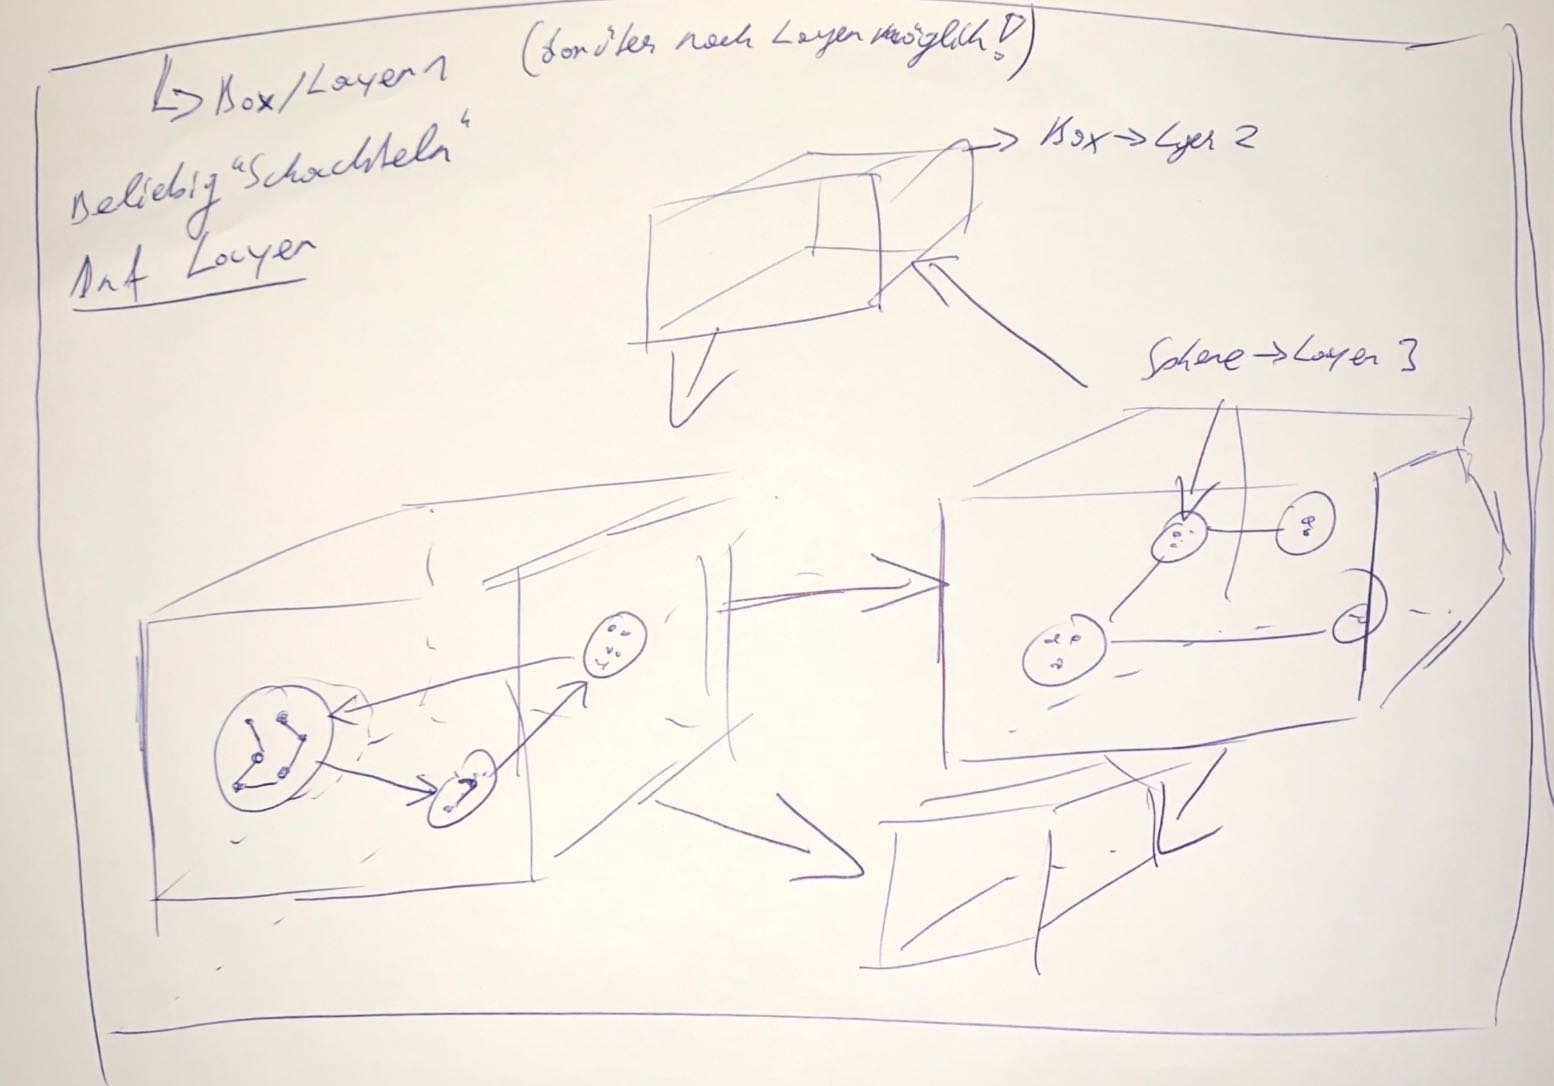
\includegraphics[width=1\textwidth]{chapters/graphics/concept1.jpg}
    \caption{(TODO redraw sketch)A sketch of our preferred layout. } 
    \label{fig:layoutSketch} 
\end{figure}

The main goal is to prevent overlapping of nodes while still visualize the different clusters of hierarchical nodes by proximity. Figure \ref{fig:layoutSketch} shows a sketch of our envisioned layout. The whole data can be seen as a tree structure where each entity in the tree is a graph itself nested in its parent node. Therefore, the number of nodes can grow exponentially with the number of hierarchical layers. Note that the root node is not displayed because it would just create an additional complexity in the visualization without adding any meaningful benefit.

\subsection{Layout Forces and Constraints}
We developed a system of multiple forces and constrains to automatically calculate the positions of all nodes. We want to achieve an evenly distributed graph while still fulfilling the rules we set ourselves for hierarchical nesting. Firstly we define a set of force and constraint templates:
\begin{itemize}
    \item ManyBody-Force: This force is a repulsion force and causes nearby nodes to push each other off. The strength decreases with the distance of the nodes. This allows the distribution of nodes evenly among the available space.
    \item Link-Force: It is the counterpart of the ManyBody-Force and pulls nodes connected via a link closer together. Together with the ManyBody-Force it enables us to model a distributed graph while still clustering connected nodes and minimizing the chance for a link to cross a not involved node.
    \item Collision-Force: This force is basically a reinforced version of the ManyBody-Force it prevents nodes from overlapping in the case the ManyBody- and Link-Force push nodes into each other.
    \item Spherical-Constraint: The spherical-constraint is the core concept of our layout we use for nesting nodes. It allows us to “squish” multiple nodes in a sphere for any given point and radius. The center of the sphere can variate for each simulation step. The constraint works by constantly adding a slightly randomized velocity for each node towards the center of the sphere. If the node is outside the sphere, then the velocity is increased drastically.
    \item Center-Force: This force helps us to position the entire visualization in the center of our viewpoint, however there is no strict distance or radius like the Spherical-Constraint applies.
\end{itemize}

It is important to understand that these templates are not applied equally to all nodes. Instead, we apply multiple instances of these forces with different parameters to subsets of our graph. 
This separation allows us to prevent of interference between different group of nodes for different parents.\\ 
Firstly we distinguish between the top hierarchical layer, from now on called layer $0$, and all other subsequent layers 1,2,3 and so on. Each node and link instance is assigned their respectively layer attribute. Layer $0$ is treated separately because these nodes have no direct assigned parent node. 
For Layer $0$, the center-force with the coordinates $(x:0,y:0,z:0)$, ManyBody-Force, Collision-Force and lastly Link-Force are applied to all nodes and links with a layer $0$ attribute. 
As for layer $1$ to layer $n$, we do not apply forces by layer but instead by parent node. For each parent we add a Collision-force, ManyBody-force and Link-force for all child nodes and links. In addition, the Spherical-Constraint is also added for all child nodes with the position of the parent node as a center. Note that the position of the parent node can change each simulation iteration, so we also update the center position for that specific constraint entity.\\
In conclusion, the total number of forces and constraints in our force system is: 
\begin{equation}
    |forces| + |constraints| \: = 4 \, + 4 * |parent\_nodes|
\end{equation}

\subsection{Stability of the force system}

A big challenge in our force system was to equally balance out all added forces so that each one performs their specific task and does not influence the effect of other forces. To achieve that, we parameterized each force with a strength parameter.
In addition, we also use the concept of an alpha Target from D3.js \cite{bostock_d3js_nodate}. To put it briefly, it is an additional value which decreases throughout the simulation this allows the simulation to “cool down” and stop it as soon as it reaches that set alpha Target value. We use the alpha Target to control the number of simulation interations. 
Besides balancing out the different templates of forces we also have to decrease the strength recursively for each layer as the nodes and their radius get smaller each layer iteration.\\
To further improve the stability of the layout, we add a small amount of randomness to the applied velocities and strengths. This improves the nodes distribution and prevent scenarios where multiple nodes receive the same forces and therefore overlap each other.\\
During our optimization we stumbled upon the problem that nodes tend to jump rapidly to a far position. This is only natural as we squish the nodes into the sphere of the parent while still applying the ManyBody- and Collision-Forces. Therefore, in some boundary scenarios the only “free” position for this node is further away which results in the jumping behavior. However, it defeats the concept of successively fine-tuning the positions throughout the simulation steps. For example nodes of layer 1-3 would be already positioned well but in the last simulation step the parent node in layer 0 would jump and therefore layer 1-3 nodes are positioned outside the parent layer 0 node again. To circumvent that problem, we do not perform the positioning of all nodes throughout the entire simulation, instead we split up the amount of simulation steps and perform them for each layer successively (see Figure \ref{fig:SimulationSteps}). Beginning with positioning the layer 0 nodes afterwards layer 1 nodes and so on. Luckily, we also gain a performance benefit through that strategy. The reason for this is that the number of nodes grows exponentially for each layer, now that we only perform a subset of the simulation interactions to that increasing number of nodes the sum of position update operations reduces significantly.
\begin{figure}[h]
    \centering
    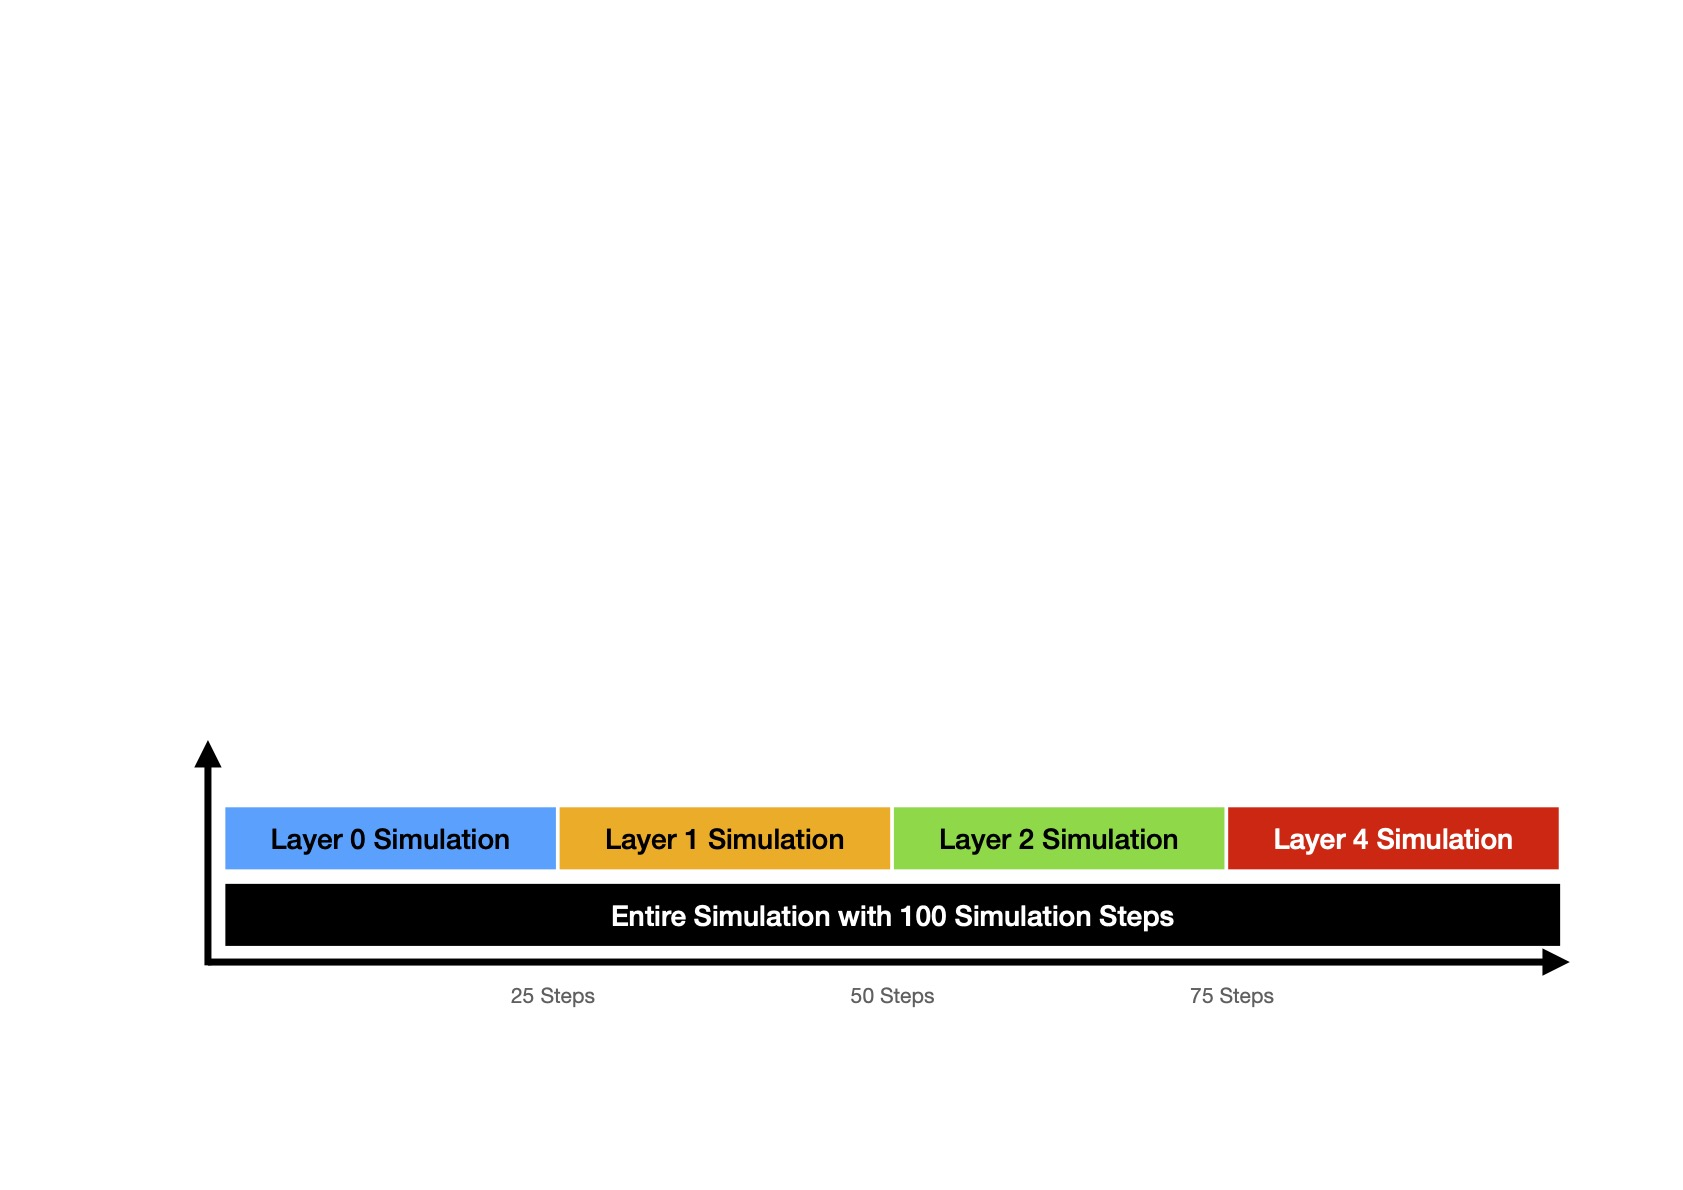
\includegraphics[width=\textwidth, trim={5cm 5cm 0 25cm},clip]{graphics/simulationStepsSplit.jpg}
    \caption[Optional caption for the figure list (often used to abbreviate long captions)]{Distribution of all simulation steps for a dataset with 4 hierarchical layers. Each layer receives the same amount of simulation steps, in this case 25 from 100.} % Remove the [...] argument if the original caption should be used in the figure list.
    \label{fig:SimulationSteps} 
  \end{figure}
\section{Graph Representation}
The goal of the graph representation was to choose appropriate rendering methods which allow us to reduce visual clutter and improve clarity while still displaying as much data as possible.\\
To represent the graph data, we choose spheres for nodes, tubes as links and cones as arrow heads indicating the link direction.
With solid textures the overview ability of the visualization would be poor since our layout approach use nested layers and therefore the user could only see one layer of nodes at the same time. To circumvent that we render all nodes transparent, then the user is able to see the nested nodes inside its parent node(TODO Figure). 
However, links inside other nodes are not visible because displaying a huge number of links would rather increase visual clutter and reduce overview. To deal with the big amount of links we apply filter conditions which are described in Section \ref{chap:ps-filterLinks}.
During the entire visualization process that the user should be able to detect the borders of the nodes and their hierarchical nesting.\\ Now that our nodes are transparent, it would be hard to detect if a another node is nested in the current parent node the camera is placed into or not. Therefore, we render a wireframe (TODO Figure) with the help of the improved spatial impression given by the virtual reality room scale experience this allows the user to better see the border of node. To further improve the assignability of nodes to their layers each node and link of the same layer shares a predefined color.\\
Of course an important part of the visualization process is to display names and details for nodes. To this end, each node instance has a billboard text label which is placed on the border of the node and always points to the camera.

To ensure an equal down scaling of all rendered entities as well as correcting the needed node radius for the layout forces we use a visualization wide scaling factor:
\begin{equation}
    scalingFactor = \frac{1}{(layer+1)^{(layer+1)} * constant}
\end{equation}

We also take the number of child nodes into account when calculating the node size: 

\begin{equation}
    nodeSize = baseSize + (numChildNodes * constant)
\end{equation}

\section{Interaction}
\label{chap:solution-interaction}

Every interactive visualization needs methods to interact with the data. 
For our visualization the requirements are that the user is able fr 

\begin{figure}[h]
    \centering
    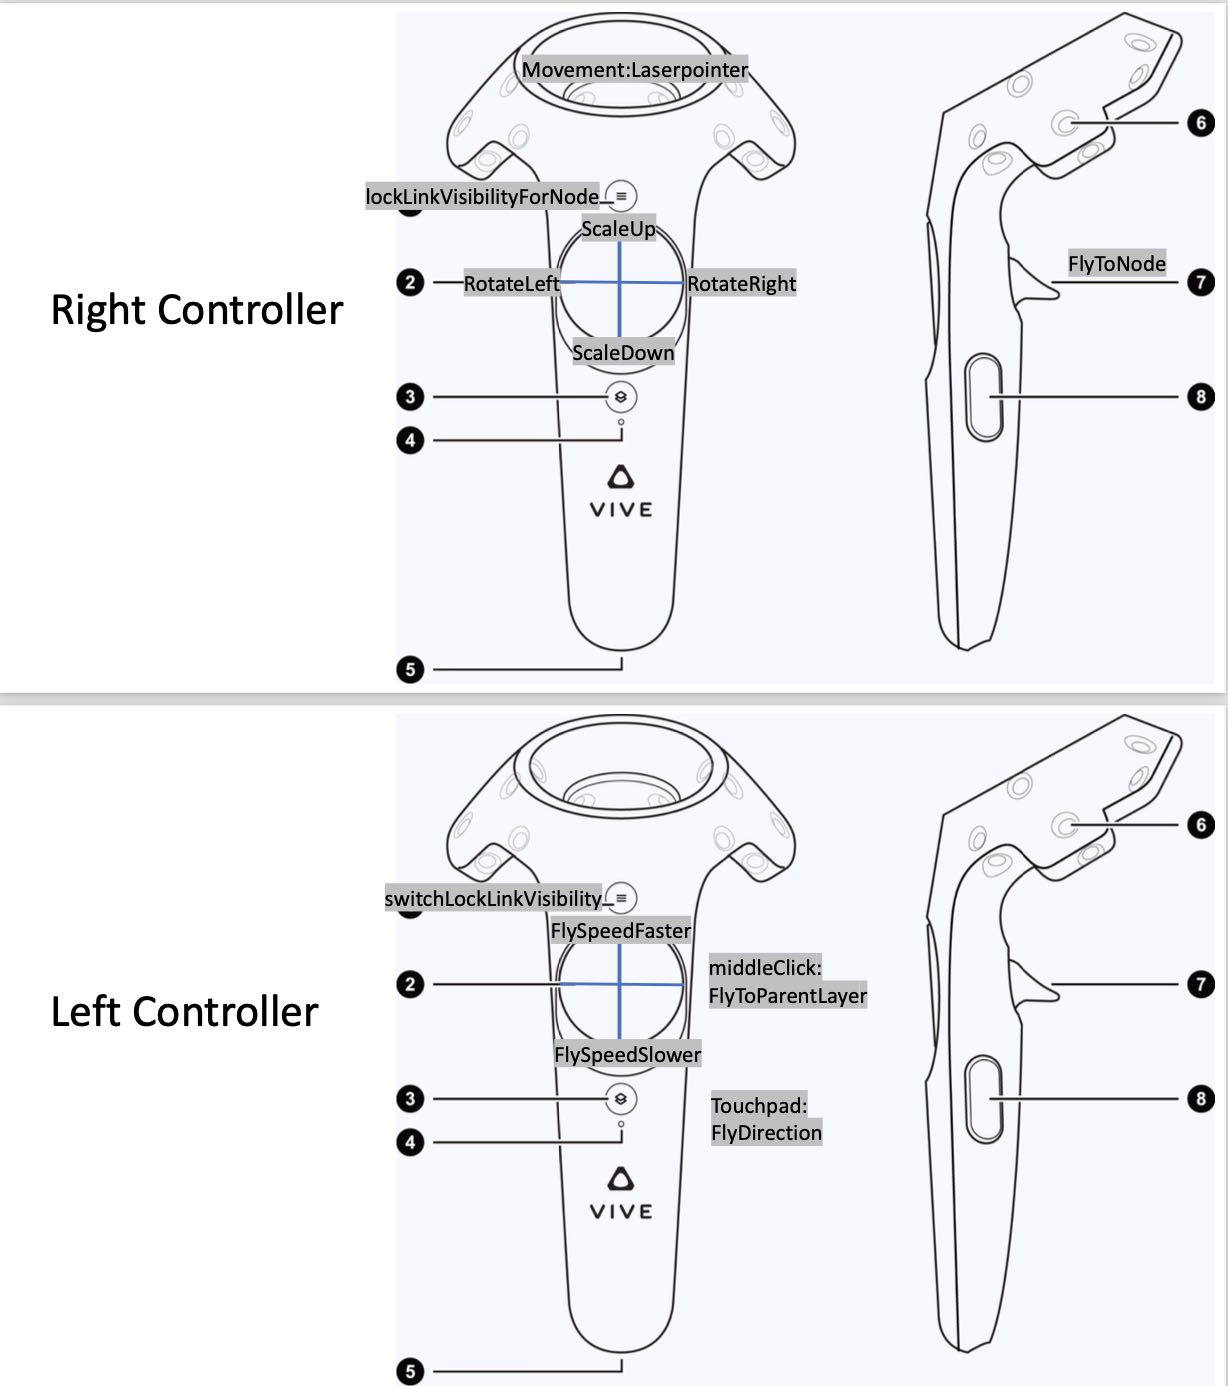
\includegraphics[width=1\textwidth]{chapters/graphics/controllerMapping.jpg}
    \caption{(TODO redo sketch)Controller mapping.} 
    \label{fig:controllerMapping} 
\end{figure}

%End of Section or Implementation
We optimized our application for the HTC Vive therefore all described button mappings refer to the HTC Vive controllers. However, we only use simple buttons, trackpads and industry standard tracking methods. 
As other 6-DOF headsets usually provide the same or similar interaction possibilities, the interaction concept of our visualization can be applied to other headsets as well.\\

Figure \ref{fig:controllerMapping} provides an overview of all available interaction methods in our application. Multiple interactions require the selection of a node beforehand, to this end we implemented the common concept of ray cast selection. 
Along the length of the right controller a ray cast is performed throughout the scene. To better visualize the effect we render a straight red line to imitate a virtual laser pointer.
The first intersected node is used as the selected node for other interaction methods like filtering or teleportation. The id and name attribute of the selected node is displayed in a HUD element centered in the lower part of the screen inside the headset. In addition, the selected node is visually highlighted through graying out the other nodes to increase the contrast. This allows the users to quickly see which node they currently have selected.

An interesting aspect of the Vive controllers (see Figure \ref{fig:controllerMapping}) is that the grip buttons (nr. 8) on both sides of the controller are actually only one button instead of two. The reason for that is that the controller is designed to fit both hands. 
So in summary we can only use 3 buttons on each controller: the trigger (nr. 7), menu button (nr. 1) and a click on the trackpad (nr. 2). The system button (nr. 3) can not be used by an application as it opens the Steam overlay settings. To stretch the number of available buttons we used the clicking position of the trackpad. This allows us to have 5 virtual buttons on the trackpad: top, bottom, left, right and center. An advantage of this method is also that these virtual buttons can be used fluently while also interacting with the touch sensitive trackpad at the same time by one finger. 

\subsection{Filtering Link Visibility}
\label{chap:ps-filterLinks}
A common technique in the visualization domain is that of details or filtering on demand. We apply this concept to reduce the visual clutter produced by overlapping of multiple links.\\
The filtering is always applied and can not be turned off. It refers to a specific selected node which then is used in the filter function.\\
To select that node there are two modes. Firstly an automatic mode which uses the current position of the users in particular the position of the headset e.g. the “camera” in the scene. 
The innermost node is selected by default for filtering, in addition the user can lock the selected node with the button “switchLockLinkVisibility” on the controller (see Figure \ref{fig:controllerMapping}). This prevents the selected node to change as the user moves around the scene, this lock can be disabled by a press on the same button.
Secondly there is a manual mode to select a specific node by using the laser pointer and pressing the “lockLinkVisibilityForNode“ button on the controller. When selecting a specific node via this method, the lock from the automatic mode is automatically set to prevent change when moving around.\\
The filter function now uses that selected node to calculate which links are visible and which not. The rules for the function are the following:
\begin{itemize}
    \item If none node is selected and the user is not inside any node only the links from the top layer 0 are displayed.
    \item All links with source or target of that selected node are displayed. 
    \item All links with source or target of direct child nodes from the selected nodes are displayed. Direct child here means the hierarchical child one layer below the selected node. 
    \item All other links are not visible.
\end{itemize}

In an earlier version we not only displayed the links of direct child nodes but instead links of all recursively child nodes. However, this quickly leads to visual clutter therefore we stuck to the direct child approach.

\section{Navigation}
\label{chap:solution-navigation}

There are two modes for navigation implemented in the application: a free-fly and a teleport technique.\\
To perform small adjustments in position, especially when the users free space is limited, the user can freely fly in the virtual scene. To control the direction the left touch sensitive trackpad can be used. 
The forward direction is linked to the users gaze direction, so the final fly direction is the combination of gaze direction and trackpad touch position. 
In addition, the fly speed is adjustable with a click on top or bottom of the trackpad.    
Similar to other VR applications we also implemented a camera rotation. This allows the users to better position themselves in the real world, particular with cable bound headsets this is useful because multiple rotations in the real world require to step over the cable. In other VR applications the movement is usually done with the left controller and rotation with the right, analogue to Gamepad controls in most games. Therefore, we mapped the rotation to the right trackpad by clicking either on the left or right corner.

For covering long distances and navigate through the hierarchical layers we implemented an animated teleportation method. The user can select a node by the laser pointer and then press the right trigger (nr. 7) to initiate the teleportation. The target position is the closest edge barely inside the node, this allows the user to get an overview of the entire nodes and links in that selected node.   
As with a simple teleportation the hierarchical aspect of the graph would lead to confusion, we perform a short animation to the target position. The speed of the animation is done with an ease-in and ease-out transition.
Remember that as soon as the users enters another node, no matter if this happens during teleportation or free flying, the visibility of links changes, provided there is no active lock.\\
Instead of teleporting deeper into the hierarchical networks the user can also teleport to the parent hierarchical layer. In particular to the edge barely outside the node the user is currently located in, this teleportation can be triggered by pressing the middle of the left trackpad.\\
All teleportation methods can be freely combined even during the animation, therefore allowing the user to fluently move around the graph. 
To further improve the overview we display the current hierarchical layer e.g. “layer: 2/5“ as a text element floating over the right controller. 

\subsection{Challenge of spatial reference in VR}

A challenge of our hierarchical layout is that nodes and links are exponentially getting smaller each hierarchy step. 
2D visualization usually deal with that by adjusting the viewport of the visualization e.g. zoom in and out. 
However, in the context of a 3D VR visualization a simple zooming approach is not possible. 
In a 3D non VR visualization that problem can be mitigated by adjusting the movement speed. Therefore, distances seem similar in size for the inner nodes and navigation is also possible without overshooting the target position.\\ 
VR visualization are trickier due to the spatial impression by rendering two perspectives. On a 2D projected image like a normal computer screen distances in the scene can only be estimated through movement. From a static image the human eye is not able to recognize the distance or size of an object without any additional size reference. 
In the real world however we constantly see objects from two different perspectives as we have two eyes, this enables the human mind to estimate distances without the need of any movement. VR works the same way by rendering the scene from two different perspectives each for one eye.  
This means that a simple trick of adjusting the movement speed is not working for our VR visualization. 
That problem makes itself noticeable for example as layer 4 nodes in VR are the size of a finger where layer 0 nodes are these of the entire room.
In addition to the perspective problem changing the movement speed also do not work because movement in a 6-DOF VR headset is also always done by movement in the real world and obviously the physical movement speed can not be adjusted.

The only real solution to that problem in our opinion is scaling the entire scene. Therefore, we implemented two techniques in our visualization:
\begin{itemize}
    \item Dynamically adjust the fly speed while navigating in the graph. On entering a node the speed slows down when leaving speeds up again. 
    \item Dynamically scaling the entire scene. When teleporting to a node in a deeper hierarchy layer, an upscaling transition is started. On teleporting to the parent layer a downscaling transition is started. 
\end{itemize} 

In addition, the scale can also be manually changed by the user at any time by pressing the upper or lower corner of the right trackpad. 
This is important as we can not know the available room space of the users VR setup. Therefore, the scale can not be optimized beforehand for a walking experience. The manual scaling gives the users the ability to adjust the scale to their liking.
%Problem Größenbezug real world + virtual scene\\
%1. Dynamischen fly speed\\
%2. Dynamisches skalieren\\
%manueller speed + skalierung wichtig da nicht klar was User preferred und wie groß sein space ist\\ 
\section{Exploration Flow}
To provide an optimal exploration experience of the hierarchical network we use the visual information seeking mantra \ref{seeking mantra}. 
At the beginning the user is in the overview perspective. He/she is placed on a further position away from the center where a good look on the entire graph is possible, in addition rotation to the graph can be applied.
When the user decides to dive deeper in the network, a node can be selected via the ray cast controller interaction. This triggers the transition into the detail perspective. 
Here all navigation and interaction methods described in Section \ref{chap:solution-interaction} and \ref{chap:solution-navigation}
are available. 
A core concept for the exploration in the detail perspective is the use of the VR room-scale navigation experience. As the user is able to tweak the scale of the scene to their liking, walking around the graph is possible for different room sizes. The goal is to improve spatial impression of the graph which results in a better clarity and understanding of the data.

TODO abschluss vom chapter